\documentclass[english]{article}
\usepackage[T1]{fontenc}
\usepackage[utf8]{luainputenc}
\usepackage{graphicx}
\usepackage{babel}
\usepackage{xcolor}
%Gummi|065|=)
\title{\textbf{GIF++ DAQ based on DIM}}
\author{L.Mirabito}
\date{}
\begin{document}

\maketitle
\section{Slow Control}
\subsection{Processes configuration}
The processes are driven via a unique daemon running on each connected PC called the job control. It's a dim server that has to be started once on each considered computer. If one computer crash it's the only needed process to restart.
\subsubsection{DimJobControl}

On each slow control computer the process is started by
\begin{verbatim}
sudo /etc/init.d/dimjcd start
\end{verbatim}
The usual stop and status options are available.

\subsubsection{Controlling slow control process}

A DimJobInterface program allows to start and stop process on all connected computer via the DimJobControl daemon. It is based ona JSON description of the needed process.

Here is the one used at GIF++ in August 2015. The structure is simple and self-describing.


\begin{verbatim}
{
    "hosts" :
    {
        "lyosdhcal11":[
            {
            "Name":"CAENSERVER",
                "Arguments" : ["-f /data/NAS/toto.slcio","-c MONCOLLECTOR"],
            "Environnement" : [
                "DIM_DNS_NODE=lyosdhcal11",
                "SLOWDB=acqilc/RPC_2008@lyosdhcal11:GIFPP2015;GIFLYON2",
                "LD_LIBRARY_PATH=/usr/lib:/usr/local/lib:/opt/dhcal/lib:/opt/dhcal/DQM4HEP/lib:/opt/dhcal/dim/linux:$LD_LIBRARY_PATH"
            ],
            "Program" : "/opt/dhcal/bin/dimcaenhv"
            }         
        ],
        "lyoilcrpi24":[
            {
            "Name":"BMP183SERVER",
                "Arguments" : ["-f /data/NAS/toto.slcio","-c MONCOLLECTOR"],
            "Environnement" : [
                "DIM_DNS_NODE=lyosdhcal11",
                "LD_LIBRARY_PATH=/usr/lib:/usr/local/lib:/opt/dhcal/lib:/opt/dhcal/DQM4HEP/lib:/opt/dhcal/dim/linux:$LD_LIBRARY_PATH"
            ],
            "Program" : "/opt/dhcal/bin/dimbmp183"
            }         
        ],
// Test avec 2 programmes
        "lyoilcrpi02":[
            // GPIO
            {
                "Name":"GPIOSERVER",
                "Arguments" : [],
                "Environnement" : [
                    "DIM_DNS_NODE=lyosdhcal11",
                    "LD_LIBRARY_PATH=/usr/lib:/usr/local/lib:/opt/dhcal/lib:/opt/dhcal/DQM4HEP/lib:/opt/dhcal/dim/linux:$LD_LIBRARY_PATH"
                ],
                "Program" : "/opt/dhcal/bin/dimgpio"
            },
            // DS1820
            {
                "Name":"DS1820SERVER",
                "Arguments" : [],
                "Environnement" : [
                    "DIM_DNS_NODE=lyosdhcal11",
                    "LD_LIBRARY_PATH=/usr/lib:/usr/local/lib:/opt/dhcal/lib:/opt/dhcal/DQM4HEP/lib:/opt/dhcal/dim/linux:$LD_LIBRARY_PATH"
                ],
                "Program" : "/opt/dhcal/bin/dimds1820"
            }          
        ]
    }
}

\end{verbatim}

The DimJobInterface belongs to the python package Ldimjc. It has few methods to start, stop and list processes belonging to the description file.
\subsubsection{Usage}
On lyosdhcal11 with DIM\_DNS\_NODE correctly defined the DimJobInterface is instantiated in python with
\begin{verbatim}
>>>import Ldimjc
>>> dsc=Ldimjc.DimJobInterface()
\end{verbatim}

Then a set of commands allows to control the process:
\begin{itemize} 
\item \textcolor{red}{ \bf  import Ldimjc} :  imports the python package

\item \textcolor{red}{\it \bf dsc=Ldimjc.DimJobInterface()}: It creates the interface 

\item \textcolor{red}{\it \bf dsc.loadJSON("slow\_conf.json")}: It loads and parses the given files, scan the DNS to have the list of DimJobControl daemon   

\item \textcolor{red}{\it \bf dsc.startJobs("lyoilcrpi02")}: it starts the jobs described in the configuration on the given host. If the host is "ALL", theb all the jobs desribed in the file are started. 
\item \textcolor{red}{\it \bf dsc.clearHostJobs("lyoilcrpi02"}: it kills all the jobs started on lyoilcrpi02 or on any host given
 \item \textcolor{red}{\it \bf dsc.clearAllJobs()}: it kills all jobs on all hosts
\item \textcolor{blue}{\it \bf dsc.status()}: it queries the status of all the jobs on all hosts.
\item \textcolor{blue}{\it \bf dsc.List()}: it prints the last queried status
\item \textcolor{blue}{\it \bf dsc.killJob("lyoilcrpi02",2934,9)}: it kills the job with PID 2934 on host lyoilcrpi02 with signal 9. The host and PID is found with the previous List command

\item \textcolor{blue}{\it \bf dsc.restartJob("lyoilcrpi02","DS1820SERVER",2934, 9)}: it sends a killJob message to PID 2934 on lyoilcrpi02 with signal 9 and restart the process described on this host as DS1820SERVER in the configuration file.


\end{itemize} 
\subsection{Slow control database}

\subsubsection{Construction tables}
The geometry and connection of a given setup is described with the following tables. HVRACK, DIFs,ASUs and CHAMBERs are registered in separated tables, then DETECTORs are assembly of those devices with SETUP reference. Giving a SETUP name leads to a unique list of detectors and positions
\begin{verbatim}
mysql> desc SETUP;
+-------+-------------+------+-----+-------------------+-----------------------------+
| Field | Type        | Null | Key | Default           | Extra                       |
+-------+-------------+------+-----+-------------------+-----------------------------+
| IDX   | int(11)     | NO   | PRI | NULL              | auto_increment              |
| NAME  | varchar(50) | YES  |     | NONE              |                             |
| START | timestamp   | NO   |     | CURRENT_TIMESTAMP | on update CURRENT_TIMESTAMP |
| VALID | tinyint(1)  | YES  |     | 1                 |                             |
+-------+-------------+------+-----+-------------------+-----------------------------+
mysql> desc HVRACK;
+----------+-------------+------+-----+---------+----------------+
| Field    | Type        | Null | Key | Default | Extra          |
+----------+-------------+------+-----+---------+----------------+
| IDX      | int(11)     | NO   | PRI | NULL    | auto_increment |
| HVTYPE   | int(11)     | YES  |     | 0       |                |
| HOSTNAME | varchar(50) | YES  |     | NONE    |                |
| USERNAME | varchar(50) | YES  |     | NONE    |                |
| PWD      | varchar(50) | YES  |     | NONE    |                |
| VALID    | tinyint(1)  | YES  |     | 1       |                |
+----------+-------------+------+-----+---------+----------------+
mysql> desc DIF;
+----------+-------------+------+-----+---------+----------------+
| Field    | Type        | Null | Key | Default | Extra          |
+----------+-------------+------+-----+---------+----------------+
| IDX      | int(11)     | NO   | PRI | NULL    | auto_increment |
| NUMBER   | int(11)     | YES  |     | 0       |                |
| FIRMWARE | varchar(50) | YES  |     | NONE    |                |
| VALID    | tinyint(1)  | YES  |     | 1       |                |
+----------+-------------+------+-----+---------+----------------+
mysql> desc ASU;
+--------+-------------+------+-----+---------+----------------+
| Field  | Type        | Null | Key | Default | Extra          |
+--------+-------------+------+-----+---------+----------------+
| IDX    | int(11)     | NO   | PRI | NULL    | auto_increment |
| NAME   | varchar(50) | YES  |     | NONE    |                |
| TYPE   | int(11)     | YES  |     | 0       |                |
| NASICS | int(11)     | YES  |     | 0       |                |
| VALID  | tinyint(1)  | YES  |     | 1       |                |
+--------+-------------+------+-----+---------+----------------+
mysql> desc CHAMBER;
+-------+-------------+------+-----+-------------------+-----------------------------+
| Field | Type        | Null | Key | Default           | Extra                       |
+-------+-------------+------+-----+-------------------+-----------------------------+
| IDX   | int(11)     | NO   | PRI | NULL              | auto_increment              |
| NAME  | varchar(50) | YES  |     | NONE              |                             |
| TYPE  | int(11)     | YES  |     | 0                 |                             |
| X0    | double      | YES  |     | 0                 |                             |
| X1    | double      | YES  |     | 0                 |                             |
| Y0    | double      | YES  |     | 0                 |                             |
| Y1    | double      | YES  |     | 0                 |                             |
| START | timestamp   | NO   |     | CURRENT_TIMESTAMP | on update CURRENT_TIMESTAMP |
| VALID | tinyint(1)  | YES  |     | 1                 |                             |
+-------+-------------+------+-----+-------------------+-----------------------------+

mysql> desc DETECTOR;
+-----------+------------+------+-----+-------------------+-----------------------------+
| Field     | Type       | Null | Key | Default           | Extra                       |
+-----------+------------+------+-----+-------------------+-----------------------------+
| IDX       | int(11)    | NO   | PRI | NULL              | auto_increment              |
| CHAMBERID | int(11)    | YES  |     | 0                 |                             |
| SETUPID   | int(11)    | YES  |     | 0                 |                             |
| HVRACKID  | int(11)    | YES  |     | 0                 |                             |
| HVCHANNEL | int(11)    | YES  |     | 0                 |                             |
| DIFID0    | int(11)    | YES  |     | 0                 |                             |
| DIFID1    | int(11)    | YES  |     | 0                 |                             |
| DIFID2    | int(11)    | YES  |     | 0                 |                             |
| ASUID00   | int(11)    | YES  |     | 0                 |                             |
| ASUID10   | int(11)    | YES  |     | 0                 |                             |
| ASUID20   | int(11)    | YES  |     | 0                 |                             |
| ASUID01   | int(11)    | YES  |     | 0                 |                             |
| ASUID11   | int(11)    | YES  |     | 0                 |                             |
| ASUID21   | int(11)    | YES  |     | 0                 |                             |
| PREF      | double     | YES  |     | 0                 |                             |
| TREF      | double     | YES  |     | 0                 |                             |
| VREF      | double     | YES  |     | 0                 |                             |
| Z0        | double     | YES  |     | 0                 |                             |
| Z1        | double     | YES  |     | 0                 |                             |
| HEURE     | timestamp  | NO   |     | CURRENT_TIMESTAMP | on update CURRENT_TIMESTAMP |
| VALID     | tinyint(1) | YES  |     | 1                 |                             |
+-----------+------------+------+-----+-------------------+-----------------------------+

\end{verbatim}

One has to notice in the DETECTOR table, 3 files PREF,TREF,VREF where the reference pressure, temperature and voltage are stored. They will  be used in the regulation procedure.
\subsubsection{Monitoring tables}

Each monitoring devices has its own monitoring table where measurements are stored with a time stamp:
\begin{verbatim}
mysql> desc HVMON;
+-----------+------------+------+-----+-------------------+-----------------------------+
| Field     | Type       | Null | Key | Default           | Extra                       |
+-----------+------------+------+-----+-------------------+-----------------------------+
| IDX       | int(11)    | NO   | PRI | NULL              | auto_increment              |
| HVRACKID  | int(11)    | YES  |     | 0                 |                             |
| HVCHANNEL | int(11)    | YES  |     | 0                 |                             |
| VSET      | double     | YES  |     | 0                 |                             |
| VMON      | double     | YES  |     | 0                 |                             |
| IMON      | double     | YES  |     | 0                 |                             |
| STATUS    | int(11)    | YES  |     | 0                 |                             |
| HEURE     | timestamp  | NO   |     | CURRENT_TIMESTAMP | on update CURRENT_TIMESTAMP |
| VALID     | tinyint(1) | YES  |     | 1                 |                             |
+-----------+------------+------+-----+-------------------+-----------------------------+
mysql> desc DS1820MON;
+-------+------------+------+-----+-------------------+-----------------------------+
| Field | Type       | Null | Key | Default           | Extra                       |
+-------+------------+------+-----+-------------------+-----------------------------+
| IDX   | int(11)    | NO   | PRI | NULL              | auto_increment              |
| TIN   | double     | YES  |     | 0                 |                             |
| TOUT  | double     | YES  |     | 0                 |                             |
| HEURE | timestamp  | NO   |     | CURRENT_TIMESTAMP | on update CURRENT_TIMESTAMP |
| VALID | tinyint(1) | YES  |     | 1                 |                             |
+-------+------------+------+-----+-------------------+-----------------------------+
mysql> desc PTMON;
+-------------+------------+------+-----+-------------------+-----------------------------+
| Field       | Type       | Null | Key | Default           | Extra                       |
+-------------+------------+------+-----+-------------------+-----------------------------+
| IDX         | int(11)    | NO   | PRI | NULL              | auto_increment              |
| PRESSURE    | double     | YES  |     | 0                 |                             |
| TEMPERATURE | double     | YES  |     | 0                 |                             |
| HEURE       | timestamp  | NO   |     | CURRENT_TIMESTAMP | on update CURRENT_TIMESTAMP |
| VALID       | tinyint(1) | YES  |     | 1                 |                             |
+-------------+------------+------+-----+-------------------+-----------------------------+

\end{verbatim} 

\subsection{Control and Measure}
Each of the process described in the slow\_conf.json configuration file is controlling a different hardware:
\begin{itemize}
\item {\bf CAENSERVER }: it runs on lyosdhcal11 and connects the mysql database specified in the SLOWDB variable. The SETUP used in the GIFPP2015 database is GIFLYON2 in this case. On initialise it queries the detector connected, the corresponding HVRACK and connect to the CAEN SY1527 specified there. It uses the SETUP to monitor and/or regulate the detector channels. It provides also single channel access to change manually high voltage and current limit. 

\item {\bf GPIOSERVER}: it runs on lyoilcrpi02 and controls the switch of the low voltage power supplies of the SDCC VME card and of all the DIFs

\item {\bf DS1820SERVER}: it runs on lyoilcrpi02 adn read 2 DS1820 temperature probes. The first one is in the box, the second is on the detector rack. The periodicity of the readout is available and data can be store in the mysql database in the table DS1820MON

\item {\bf BMP183SERVER}: it runs on lyoilcrpi24 that is connected outside the zone near the SY1527 rack. It measure the pressure and the temperature with a BMP183 Bosch device. Once again the periodicty of the readout can be controlled and the data can be stored in the mysql database in the PTMON table
\end{itemize}

Once again a python package LMainSlowControl is available to control all those processes:
\begin{itemize}
\item \textcolor{red}{ \bf  import LMainSlowControl} :  imports the python package
\item \textcolor{red}{d=LMainSlowControl.DimSlowControl("lyosdhcal11.cern.ch")}: it creates the interface with the DNS lyosdhcal11.cern.ch
\item \textcolor{red}{d.scandns() }: it scans the DNS and discover services 
\item \textcolor{red}{d.CAENHVInitialise("test") }: it uses the SLOWDB variable of the CAENSERVER program to access the database and query it for the given SETUP.
\item \textcolor{red}{d.CAENHVRead(48)}: it reads channel 48
\item \textcolor{red}{d.getCurrentHVChannel()}: it returns last channel read 
\item \textcolor{blue}{d.getCurrentHVVoltageRead()}: it returns last VMON read
\item \textcolor{blue}{d.getCurrentHVCurrentRead()}: it returns last IMON read
\item \textcolor{blue}{d.getCurrentHVVoltageSet()}: it returns last VSET read
\item \textcolor{blue}{d.CAENHVSetOn(49)} : turns HV on channel 49
\item \textcolor{blue}{d.CAENHVSetOff(49)}: tuns HV Off on channel 49
\item \textcolor{blue}{d.CAENHVSetVoltage(48,3300)}: it sets VSET to 3300 V on channel 48
\item \textcolor{blue}{d.CAENHVSetCurrent(48,50)}: it sets I0 to 50 microA on channel 48
\item \textcolor{blue}{d.CAENHVStartRegulation(60)}: it starts the regulation with a period of 60 s. It queries the database for each detector of the setup, looks for current Voltage, makes a mean of the last measure pressure measured by the BMP183 (PMEAN)  and last TOUT temperature measured by the DS1820 probe (TMEAN). It compares the effective voltage to the VREF recalculated from (PREF,TREF) to (PMEAN,TMEAN) and correct the voltage VSET if the differenc is bigger than 20 V and bellow 200 V
\item \textcolor{blue}{d.CAENHVStartMonitor(120)}: it reads all detector channel sepcified in the SETUP and store the in HVMON every 120 s
\item \textcolor{blue}{d.CAENHVStopRegulation()}: it stops the Regulation thread
\item \textcolor{blue}{d.CAENHVStopMonitor()}: it stops the monitroing thread
\item \textcolor{blue}{d.BMP183SetPeriod(30)}: it set the period of the BMP183 reading
\item \textcolor{blue}{d.BMP183Store("acqilc/RPC\_2008@lyoac30.cern.ch:GIFPP2015")}: it stores BMP183 data in PTMON table on the given account
\item \textcolor{blue}{d.DS1820SetPeriod(30)}: it sets the period of the DS1820 reading
\item \textcolor{blue}{d.DS1820Store("acqilc/RPC\_2008@lyoac30.cern.ch:GIFPP2015")}: it stores the DS1820 data in the DS1820MON table on the given account.
\item \textcolor{red}{d.OpenGPIO()}: it opens the GPIO access
\item \textcolor{blue}{d.VMEOn()}: turns VME LV On
\item \textcolor{blue}{d.VMEOff()}: turns VME LV Off
\item \textcolor{blue}{d.DIFOn()}: turns DIF LV On
\item \textcolor{blue}{d.DIFOff()} turns DIF LV Off
\item \textcolor{red}{d.CloseGPIO()}: closes the GPIO access

\end{itemize}
\section{DAQ Architecture}

\subsection{PC names and role}
The acquisition is based on 1 RaspberryPI micro computer controlling and reading up to 9 DIFs connected on each of the 7 planes: {\sl \bf lyoilcrpi02}. Data are collected and written to disk on the linux PC {\sl lyosdhcal11}.

The  RPI is responsible for chip configurations, DIF control and data readout. {\sl \bf lyoilcrpi02} is also handling the control of the SDCC. The central PC is in charged of the configuration database access, the data collection, the event building and writing and the human interface instance

Since DIM is the network framework used in this data acquisition, the DIM DNS must be stated once {\sl \bf lyosdhcal11} with
\begin{verbatim}
killall -9 dns
export DIM_DNS_NODE=lyosdhcal11
/opt/xdaq/bin/dns &>/dev/null &
\end{verbatim}

\subsection{DIF control}

On each RPI should run a DIM daemon that controls the DIF connected to it. It is started with

{\sl \bf sudo /etc/init.d/dimdifd start }

its status is obtained with 

{\sl \bf sudo /etc/init.d/dimdifd status }

and it can be stoped with

{\sl \bf sudo /etc/init.d/dimdifd stop }

The log file is {\sl \bf /var/log/dimdif.log }

It is a DIM server acknowledging the following commands:
\begin{itemize}
\item { \bf SCANDEVICES }: List all DIFs connected on USB and publish a DIM Service DEVICES of 255 integers with the identifiers of the found DIFs
\item {\bf INITIALISE}: requires the DIF identifier, it opens the DIF devices and tries to write and read the test register. It updates the Dim Services STATE and INFO and returns an INITIALISED state in case of success or INIT\_FAILED
\item {\bf REGISTERSTATE}: requires the control register (integer) and the current Database state (string). It stores the control register to be used at the next configuration and subscribes to the database DIM server services publishing DIF parameters for each DIF separately (/DB/{\sl STATE\_NAME}/DIF{\sl id}). By this way it obtains from the dimdb service the configuration parameter of each DIF.

\item {\bf CONFIGURE}: it configures all connected DIF and their asoociated ASICs. It updates the STATE and the INFO of each DIF. The STATE contains the whole decoding of the slow control status. 


\item {\bf START}: it starts the acquisition of each DIF. The STATE of each DIF is updated to STARTED.

\item {\bf STOP}: it stops the acquisition of each DIF. The STATE of each DIF is updated to STOPPED.

\end{itemize}

It also publishes 3 services per DIF:
\begin{itemize}
\item {\bf STATE}: a string containing the current DIF state (FOUND, INITIALISED, PRECONFIGURED, CONFIGURED, STARTED, STOPPED)

\item {\bf INFO}: a structure with {\sl dif id, status, slow control status, bcid, gtc,  bytes read and pc name}

\item {\bf DATA}: the last DIF data buffer read. 
\end{itemize}


\subsection{SDCC control}

A DIM daemon is running on the RPI ({\sl clrtorp2-prive}) where the SDCC is connected.It is started with

{\sl \bf sudo /etc/init.d/dimcccd start }

its status is obtained with 

{\sl \bf sudo /etc/init.d/dimcccd status }

and it can be stoped with

{\sl \bf sudo /etc/init.d/dimcccd stop }
 
 The log file is {\sl \bf /var/log/dimccc.log }
 
 It acknowlegdes the following commands:
 \begin{itemize}
\item {\bf INITIALISE}: requires the CCC FTDI identifier ("DCCCCC01"), it opens the SDCC devices and tries to write and read the test register. 
\item {\bf CONFIGURE}: it sends DIFRESET and CCCRESET before the start of the acquisition
\item {\bf DIFRESET}: it sends a DIFRESET command on the DCC bus
\item {\bf CCCRESET}: it send a CCCRESET command on the DCC bus
\item {\bf PAUSE}: it send a PAUSE command on the DCC bus
\item {\bf RESUME}: it send a RESUME command on the DCC bus
\item {\bf START}: it send a START\_ACQUISITION command on the DCC bus
\item {\bf STOP}: it send a STOP\_ACQUISITION command on the DCC bus
\item { \bf TESTREGISTERREAD }: read the test register and update the REGISTER DIM service
\item { \bf TESTREGISTERWRITE }: requires an integer value that is written in the test register
\end{itemize}

It publishes 2 DIM services,{\bf REGISTER} that is filled when TESTREGISTERREAD is called and an integer {\bf STATUS} which value is changed depending on the last command received.
 
\subsubsection{Possible issue}

At power on, the USB control may be faulty. It is recommended to INITIALISE and use the TESTREGISTERWRITE/READ to check the correct access of the FPGA.

\subsection{Database control}

The database control is the responsability of one DIM daemon server running on the central PC ({\bf \sl clrtodaq0-prive}.It is started with

{\sl \bf sudo /etc/init.d/dimdbd start }

its status is obtained with 

{\sl \bf sudo /etc/init.d/dimdbd status }

and it can be stoped with

{\sl \bf sudo /etc/init.d/dimdbd stop }
 
 The log file is {\sl \bf /var/log/dimdb.log }
 
 It acknowlegdes the following commands:
 \begin{itemize}
\item {\bf DOWNLOAD}: requires the name of the needed DB state ("LPCC\_230"), it downloads the given state from the configuration databas and creates for each DIF a DIM service withe name /DB/{\sl STATE\_NAME}/DIF{\sl id} containing the configuration parameters for all the ASICs of the given DIF 
\item {\bf DELETE}: it deletes all the DIM services of the current state
\item {\bf NEWRUN}: it asks the database for a new run number and update /DB/RUNFROMDB service

\end{itemize}

\subsection {Data writing}

The data writing is achieved by one DIM daemon server running on the central PC ({\bf \sl lyosdhcal11}.It is started with

{\sl \bf sudo /etc/init.d/dimwriterd start }

its status is obtained with 

{\sl \bf sudo /etc/init.d/dimwriterd status }

and it can be stoped with

{\sl \bf sudo /etc/init.d/dimwriterd stop }
 
 The log file is {\sl \bf /var/log/dimwriter.log }
 
 It acknowlegdes the following commands:
 \begin{itemize}
\item {\bf INITIALISE}: it subscribes to all possible DIF DATA and INFO services connected to the DIM DNS. It also subscribes to the RUNFROMDB service from the dimdb server. It creates an {\sl ShmProxy} instance that is spying the {\sl /dev/shm} directory for new data collected. The {\sl infoHandler} method of the server received data from the {\sl dimdif} daemon DATA services and write them in {\sl /dev/shm}
\item {\bf START}: it opens an LCIO file in {\sl /data/online/Results} using the current value of run obtained by the RUNFROMDB service. It starts the {\sl /dev/shm} spying, collects data and writes them to disk when all publishing DIF have completed the same BCID buffer.
\item {\bf STOP}: it stops the spying and closes the data file.
\end{itemize}

\subsubsection{Possible issue}

This server is still partially in development. It has to be started after the other daemons in order to be able
to collect run number and DIF data. In case of failure, please exit cleanly the daq control (see next section), restart this daemon and restart the daq control   

\section {DAQ control}

The DAQ control is done on the main console loggin on lyosdhcal11 . There is a graphical interface and it will be desribe later on but the underlying control is done by the DimDaqControl package.

\subsection{ The DimDaqControl package }
The control of the DAQ is done via { \bf \sl DimDaqControl } a standalone DIM program interfaced to python. The python package LSDHCALDimCtrl  is in {\sl /data/online/SDHCAL/DimCtrl}. The environment needs to be set properly with:

\begin{verbatim}
cd /data/online/SDHCAL/DimCtrl
export LD_LIBRARY_PATH=.:./lib:$LD_LIBRARY_PATH
python
\end{verbatim}  

Inside the python shell launched you can do the following:

\begin{enumerate} 
\item \textcolor{red}{ \bf  import LSDHCALDimCtrl} :  imports the python package

\item \textcolor{red}{\it \bf s=LSDHCALDimCtrl.DimDaqControl("gifpp")}:  creates an instance of DimDaqControl

\item \textcolor{red}{\it \bf s.scandns()}: lists all DIMServer, services and commands available on the DIM DNS  
\item \textcolor{red}{\it \bf s.initialiseWriter("/data/online/Results")}: Initialise the data writing on the given directory. It has to be done only once if the dimwriter daemon is not stopped.

\item \textcolor{blue}{\it \bf s.scan()}: sends a SCANDEVICES command to all dimdif servers and wait for DEVICES service update. It must be called once or after a destroy()


\item \textcolor{blue}{\it {\bf s.initialise()}}: sends an INITIALISE command to all DIF found previously
\item {\bf s.\_print()}: prints the status of each DIF on each dimdif server from the INFO service of each given DIF. Like the scan() command it must be called only after a scan() command

\item {\bf s.download("LPCC\_230")}: triggers the DELETE of the previous state in the DB server and the DOWNLOAD of the specified state. Since no semaphore mechanism is used in this command a 20 s delay may be needed before the data are available. It has to be called only when a new DB state needs to be downloaded or when the dimdb daemon is restarted

\item \textcolor{purple}{\bf s.registerstate(0x815A1B00,"LPCC\_230")}: send a REGISTERSTATE command to all dimdif server. The state specified should be identical to the last downloaded state in dimdb. It must be called before configure to also set the control register.

\item \textcolor{purple}{\bf s.configure()}: sends a CONFIGURE command to all dimdif servers




\item \textcolor{green}{\bf s.start()}: starts a run, sends a START command to the dimccc, the dimdif and the dimwriter servers 

\item \textcolor{green}{\bf s.stop()}: stops a run,sends a STOP command to the dimccc, the dimdif and the dimwriter servers
\item \textcolor{blue}{\bf s.destroy()}: send a DESTROY command to the dimdif servers. All the DIF handling are cleared locally so the only possible next command is scan()
\end{enumerate} 

The red commands needs to be used only once per session. The blue ones should be used once or if any changes has occurred on dimdif servers (power cycle for example). The purple ones are used to reconfigure chips. The green ones are the normal one to start and stop a run. Eventually the black commands are optional, the {\bf download} one must be called at least ones to access the DB but is not needed in a new session if the dimdb server is alive and already contains the state 

\subsection{ The StartDaq package }
The {\bf \sl StartDaq} pacakge embedded the { \bf \sl DimDaqControl }  and add hosts managment, LV and HV control. It can be started directly in python on lyosdhcal11. It uses a configuration file to handle the host managment and set the DB and trigger parameter. An exemple is found in SDHCAL/python/config\_box.py:

\begin{verbatim}

host=['lyoilcrpi02']
ccc='lyoilcrpi02'
db='lyosdhcal11'
writer='lyosdhcal11'
register=0x815A1B00
# 115 + petit seup
state="GIFSPS_57"
# Novermber 2012 state="Dome_42chambres_Reference_v4_115"
# November 2012 + masks state="Dome_42chambres_Reference_v4_144"
directory="/data/NAS/GIF2015"

\end{verbatim}


Inside the python shell launched you can do the following:

\begin{enumerate} 
\item \textcolor{red}{ \bf  import StartDaq} :  imports the python package

\item \textcolor{red}{\it \bf s=StartDaq.StartDaq("config\_m3")}:  creates an instance of StartDaq withc the config\_m3.py files

\item \textcolor{red}{\it \bf s.host\_start()}: starts DIM daemon on all hosts list in config.host,config.ccc,config.db and config.writer names 
\item \textcolor{red}{\it \bf s.host\_stop()}: stops DIM daemon on all hosts list in config.host,config.ccc,config.db and config.writer names
 \item \textcolor{red}{\it \bf s.rpi\_start()}: starts DIM daemon on all hosts list in config.host
\item \textcolor{red}{\it \bf s.rpi\_stop()}: stops DIM daemon on all hosts list in config.host

\item \textcolor{red}{\it \bf s.initialiseWriter("/data/online/Results")}: Initialise the data writing on the given directory. It has to be done only once if the dimwriter daemon is not stopped.

\item \textcolor{blue}{\it \bf s.scan()}: sends a SCANDEVICES command to all dimdif servers and wait for DEVICES service update. It must be called once or after a destroy()


\item \textcolor{blue}{\it {\bf s.initialise()}}: sends an INITIALISE command to all DIF found previously
\item {\bf s.\_print()}: prints the status of each DIF on each dimdif server from the INFO service of each given DIF. Like the scan() command it must be called only after a scan() command

\item {\bf s.download("LPCC\_230")}: triggers the DELETE of the previous state in the DB server and the DOWNLOAD of the specified state. Since no semaphore mechanism is used in this command a 20 s delay may be needed before the data are available. It has to be called only when a new DB state needs to be downloaded or when the dimdb daemon is restarted

\item \textcolor{purple}{\bf s.registerstate(0x815A1B00,"GIFSPS\_57")}: send a REGISTERSTATE command to all dimdif server. The state specified should be identical to the last downloaded state in dimdb. It must be called before configure to also set the control register.

\item \textcolor{purple}{\bf s.configure()}: sends a CONFIGURE command to all dimdif servers




\item \textcolor{green}{\bf s.start()}: starts a run, sends a START command to the dimccc, the dimdif and the dimwriter servers 

\item \textcolor{green}{\bf s.stop()}: stops a run,sends a STOP command to the dimccc, the dimdif and the dimwriter servers
\item \textcolor{blue}{\bf s.destroy()}: send a DESTROY command to the dimdif servers. All the DIF handling are cleared locally so the only possible next command is scan()
\end{enumerate} 

The red commands needs to be used only once per session. The blue ones should be used once or if any changes has occurred on dimdif servers (power cycle for example). The purple ones are used to reconfigure chips. The green ones are the normal one to start and stop a run. Eventually the black commands are optional, the {\bf download} one must be called at least ones to access the DB but is not needed in a new session if the dimdb server is alive and already contains the state 


\subsection{Spying with webDid}
The latest versions of DIM provide a web interface to all DIM servers and clients. The server is started with:
\begin{verbatim}
export DIM_DNS_NODE=lyosdhcal11
/opt/dhcal/dimWebDID/webDid
\end{verbatim}

Then the interface can be accessed via a web browser at address http://lyosdhcal11:2500 as seen on figure \ref{webdid}
\begin{figure}[htp]
\centering
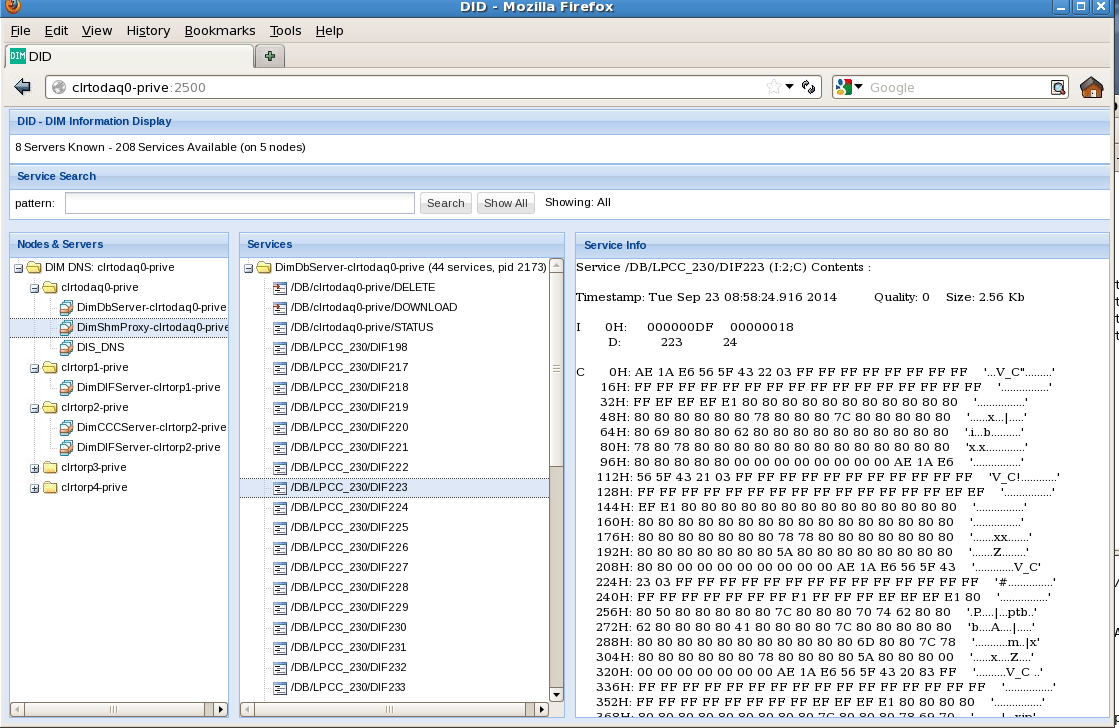
\includegraphics[width=1.3\textwidth]{./webDid.png}
\caption{The web application webDID used to spy DIM services}
\label{webdid}
\end{figure}

Commands can be sent manually but spying of dynamiclly allocated infos (like the DID DATA service) should be avoided since it crashes the program. 
\subsection{Graphical interface}
\subsubsection{Starting}
\begin{verbatim}
cd SDHCAL/python
python SDaqImpl.py
\end{verbatim}

This graphical interface is just a user friendly interface to the StartDaq package, each button corresponds to the call of one method. The figure \ref{SDaqImpl1},\ref{SDaqImpl2}, and \ref{SDaqImpl3} shows the various panel with the sequence of call of each method.
\begin{figure}[htp]
\centering
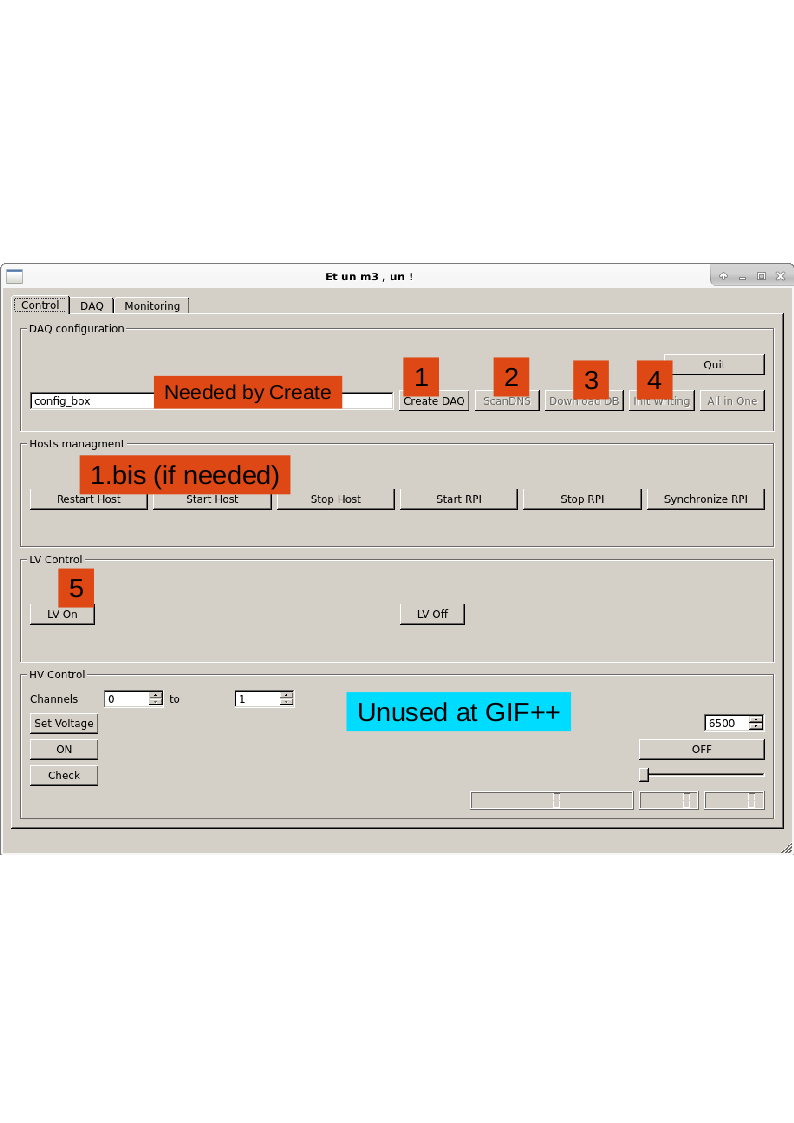
\includegraphics[width=1.\textwidth]{./SDaqImpl1.png}
\caption{Process control panel. Restart host can be called after createDaq and can be called again after a DAQ destroy but must be followed by the step 2,3 and 4}
\label{SDaqImpl1}
\end{figure}
\begin{figure}[htp]
\centering
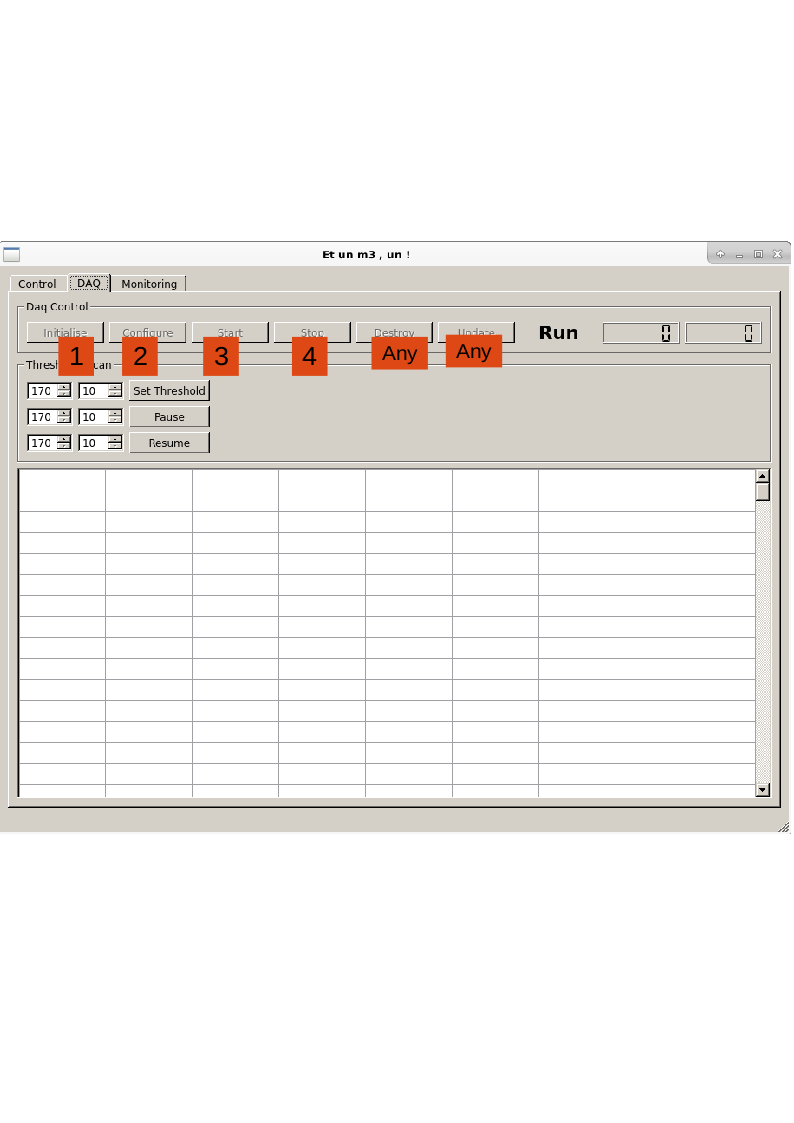
\includegraphics[width=1.\textwidth]{./SDaqImpl2.png}
\caption{Daq control panel. Initialise must be called after Destroy. After a Stop, Configure (parameter reload) or Start can be called}
\label{SDaqImpl2}
\end{figure}
\begin{figure}[htp]
\centering
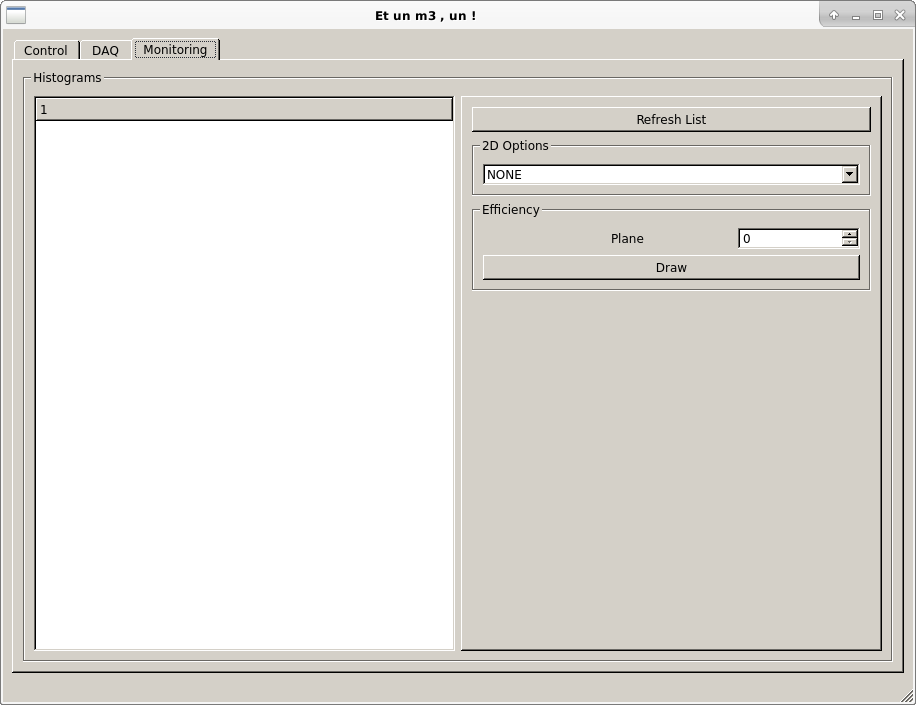
\includegraphics[width=1.\textwidth]{./SDaqImpl3.png}
\caption{Monitoring Panel. RefreshList gives the list of histograms and access to an expanding tree of histograms. Doble-clicked on a histogram to display}
\label{SDaqImpl3}
\end{figure}

\section{How to }

\subsection{Lost connection to lyoilcrpi02}

If the connection is lost to lyoilcrpi02, first check with a ping that the TCP/IP is  not answering at all:
\begin{verbatim}
ping lyoilcrpi02
\end{verbatim}

If no communication is possible go in a browser to http://lyoilcpwr01  (admin/admin) and power cycle the box. Five minutes later you should be able to connect to lyoilcrpi02
 \begin{verbatim}
ssh pi@lyoilcrpi02
\end{verbatim}

then restart the job control on it
\begin{verbatim}
sudo /etc/init.d/dimjcd start
\end{verbatim}


Now in the home of  lyosdhcal11 in python
\begin{verbatim}
import Ldimjc
dsc=Ldimjc.DimJobInterface()
dsc.loadJSON("slow_conf.json")
dsc.clearHostJobs("llyoilcrpi02")
dsc.startJobs("lyoilcrpi02")
dsc.status()
dsc.List()
# you should see the list of process
import LMainSlowControl
l=LMainSlowControl.DimSlowControl("lyosdhcal11")
l.scandns()
l.DS1820SetPeriod(30)
l.DS1820Store("acqilc/RPC_2008@lyosdhcal11:GIFPP2015")
l.OpenGPIO()
l.VMEOn()
l.DIFOn()
# wait 1 minute
l.VMEOff()
l.VMEOn()

\end{verbatim}

Keep this window open.

Now you can restart the DAQ graphical interface:
\begin{enumerate}
\item Create DAQ
\item Restart Hosts
\item Scan DNS
\item Download DB (wait 1 min)
\item Init Writing
\item LV On
\item Initialise
\end{enumerate}

After Initialise, log on lyoilcrpi02 and check /var/log/dimccc.log if the last return code is -1 that means that the USB communication to the SDCC failed and the program exited. Go in the slow control window and repeat the VME Off/On step ,then repeat the sequence

\begin{enumerate}
\item Destroy
\item Restart Hosts
\item Scan DNS
\item Download DB (wait 1 min)
\item Init Writing
\item LV On
\item Initialise
\end{enumerate}

The /var/log/dimccc.log should have return code 0 and you can now do your run.

\subsection{One DIF is in INIT\_FAILED}

That means that the USB communication cannot be established. It might be due to a connection problem (LV or HDMI) but also a SDCC issue (check again /var/log/dimccc.log)

\subsection{ One DIF cannot configured}

Check:
\begin{itemize}
\item HDMI connection
\item LV voltage on the DIF (it must be greater than 5 V)
\item DIF-ASU connector (LV Off, replug it)
\end{itemize}

If none of this fix works, it means one ASIC is faulty. There is few alternatives
\begin{enumerate}
\item Try to run: You're not sure all chips are configured and it may block the trigger
\item Keep the chamber in the setup but disable it. Unplug the LV of the DIF
\item Dismount and debug the chamber
\end{enumerate}

 
\end{document}


